\chapter{Risk Basics: Loan Default Prediction}
\label{ch:loan}

\begin{companioncode}{qf-02-loan}
Code: \texttt{crates/qf-02-loan/}\\
Dependencies: \crate{qf-common}\\
Run: \texttt{cargo run -p qf-02-loan --example loan\_analysis}
\end{companioncode}

\section{Learning Objectives}

Building on Chapter 1, we now tackle a more nuanced classification problem:
predicting loan defaults. This chapter introduces:

\begin{itemize}
    \item Feature engineering for credit risk assessment
    \item Categorical variable encoding (one-hot)
    \item Feature normalization (min-max scaling)
    \item Linear scoring models with probability calibration
    \item ROC curves and AUC---a better metric for imbalanced data
    \item Trait-based architecture in action
\end{itemize}

\begin{keyinsight}
While Chapter 1 used z-scores (a threshold on statistics), this chapter moves
toward \textbf{probability estimation}. We want to know not just ``default or
not'' but ``how likely is default?'' This probability enables better decisions
and risk-based pricing.
\end{keyinsight}

\section{Introduction: Credit Risk Fundamentals}

\marginnote{%
\textbf{Credit Risk}\\[0.3em]
The risk that a borrower will fail to repay a loan according to agreed terms.
}

When a bank issues a loan, it faces \textbf{credit risk}---the possibility that
the borrower defaults. Unlike fraud detection where we catch bad actors, loan
default prediction is about assessing the \emph{likelihood} of future failure.

Key questions in credit risk:
\begin{itemize}
    \item What factors predict default? (Feature engineering)
    \item How do we combine factors into a score? (Scoring model)
    \item How do we evaluate the score's usefulness? (ROC-AUC)
\end{itemize}

\section{Data Model}

\subsection{Loan Application Structure}

\begin{lstlisting}[language=Rust]
pub struct LoanApplication {
    pub income: f64,           // Annual income
    pub loan_amount: f64,      // Requested loan amount
    pub interest_rate: f64,    // Interest rate offered
    pub dti: f64,              // Debt-to-income ratio
    pub grade: u8,             // Credit grade (A=1 to G=7)
    pub home_ownership: HomeOwnership,
    pub defaulted: bool,       // Target: did they default?
}

pub enum HomeOwnership {
    Rent,
    Own,
    Mortgage,
}
\end{lstlisting}

\marginnote{%
\textbf{Credit Grades}\\[0.3em]
A = lowest risk\\
G = highest risk\\[0.5em]
Each grade maps to different interest rates and approval criteria.
}

\section{Feature Engineering}

\subsection{Derived Features}

Raw data rarely enters a model directly. We engineer features that capture
meaningful relationships:

\marginnote{%
\textbf{Feature Formulas}\\[0.5em]
DTI: $\dfrac{\text{debt}}{\text{income}}$\\[0.8em]
LTI: $\dfrac{\text{loan}}{\text{income}}$\\[0.8em]
Grade Score: $\dfrac{g - 1}{6}$
}

\begin{lstlisting}[language=Rust]
pub struct FeatureExtractor;

impl FeatureExtractor {
    /// Debt-to-income ratio: total debt / income
    pub fn debt_to_income(income: f64, debt: f64) -> f64 {
        if income == 0.0 { return 0.0; }
        debt / income
    }

    /// Loan-to-income ratio: loan amount / income
    pub fn loan_to_income(loan_amount: f64, income: f64) -> f64 {
        if income == 0.0 { return 0.0; }
        loan_amount / income
    }

    /// Convert grade (1-7) to risk score (0.0-1.0)
    pub fn grade_to_score(grade: u8) -> f64 {
        ((grade.saturating_sub(1)) as f64) / 6.0
    }
}
\end{lstlisting}

\subsection{Categorical Encoding}

Numerical models require numerical inputs. We encode categorical variables
using \textbf{one-hot encoding}:

\begin{center}
\begin{tabular}{lccc}
\toprule
\textbf{Home Ownership} & \textbf{RENT} & \textbf{OWN} & \textbf{MORTGAGE} \\
\midrule
Rent     & 1 & 0 & 0 \\
Own      & 0 & 1 & 0 \\
Mortgage & 0 & 0 & 1 \\
\bottomrule
\end{tabular}
\end{center}

\begin{lstlisting}[language=Rust]
pub struct OneHotEncoder;

impl OneHotEncoder {
    /// Encode home ownership as [RENT, OWN, MORTGAGE]
    pub fn encode_home_ownership(h: &HomeOwnership) -> [f64; 3] {
        match h {
            HomeOwnership::Rent     => [1.0, 0.0, 0.0],
            HomeOwnership::Own      => [0.0, 1.0, 0.0],
            HomeOwnership::Mortgage => [0.0, 0.0, 1.0],
        }
    }
}
\end{lstlisting}

\subsection{Feature Normalization}

\marginnote{%
\textbf{Min-Max Scaling}\\[0.5em]
$x' = \dfrac{x - x_{\min}}{x_{\max} - x_{\min}}$\\[0.5em]
Scales features to $[0, 1]$.
}

Different features have different scales. Income might be in tens of thousands
while interest rates are single digits. We normalize to $[0, 1]$:

\begin{lstlisting}[language=Rust]
pub struct Normalizer {
    min: Vec<f64>,
    max: Vec<f64>,
}

impl Normalizer {
    pub fn fit(data: &[Vec<f64>]) -> Self {
        // Compute min/max per feature
    }

    pub fn transform(&self, features: &[f64]) -> Vec<f64> {
        features.iter().enumerate().map(|(i, &x)| {
            let range = self.max[i] - self.min[i];
            if range == 0.0 { 0.0 } else { (x - self.min[i]) / range }
        }).collect()
    }
}
\end{lstlisting}

\section{Linear Scoring Model}

\subsection{Weighted Sum}

The simplest scoring model is a weighted linear combination:

\[
\text{score} = \sum_{i=1}^{n} w_i \cdot x_i + b = \mathbf{w}^T \mathbf{x} + b
\]

\marginnote{%
\textbf{Linear Score}\\[0.5em]
$s = \mathbf{w}^T \mathbf{x} + b$\\[0.5em]
where $\mathbf{w}$ are weights, $b$ is bias.
}

\begin{lstlisting}[language=Rust]
pub struct LinearScorer {
    weights: Vec<f64>,
    bias: f64,
}

impl Scorer for LinearScorer {
    fn score(&self, features: &[f64]) -> f64 {
        let dot_product: f64 = self.weights.iter()
            .zip(features.iter())
            .map(|(w, f)| w * f)
            .sum();
        dot_product + self.bias
    }
}
\end{lstlisting}

\subsection{Probability via Sigmoid}

The raw score can be any real number. To convert it to a probability in $[0, 1]$,
we apply the \textbf{sigmoid function}:

\marginnote{%
\textbf{Sigmoid Function}\\[0.5em]
$\sigma(x) = \dfrac{1}{1 + e^{-x}}$\\[0.5em]
Maps $(-\infty, +\infty)$ to $(0, 1)$.
}

\[
\sigma(x) = \frac{1}{1 + e^{-x}}
\]

Properties of sigmoid:
\begin{itemize}
    \item $\sigma(0) = 0.5$ (neutral score = 50\% probability)
    \item $\sigma(x) \to 1$ as $x \to +\infty$
    \item $\sigma(x) \to 0$ as $x \to -\infty$
\end{itemize}

\begin{lstlisting}[language=Rust]
/// Hand-rolled sigmoid: 1 / (1 + exp(-x))
fn sigmoid(x: f64) -> f64 {
    1.0 / (1.0 + (-x).exp())
}

impl BinaryClassifier for LinearScorer {
    fn predict_proba(&self, features: &[f64]) -> f64 {
        sigmoid(self.score(features))
    }

    fn predict(&self, features: &[f64]) -> bool {
        self.predict_proba(features) > 0.5
    }
}
\end{lstlisting}

\section{ROC Curves and AUC}

\subsection{Why Not Just Accuracy?}

\marginnote{%
\textbf{Class Imbalance}\\[0.3em]
If 95\% of loans are repaid, a model that always predicts ``no default'' has
95\% accuracy but catches zero defaults!
}

Like fraud detection, loan default is imbalanced. Accuracy is misleading.
Instead, we use the \textbf{Receiver Operating Characteristic (ROC) curve}.

\subsection{ROC Curve Construction}

The ROC curve plots \textbf{True Positive Rate (TPR)} vs \textbf{False Positive
Rate (FPR)} at various classification thresholds:

\begin{itemize}
    \item \textbf{TPR} (Recall): $\frac{TP}{TP + FN}$ --- of actual defaults, how many did we catch?
    \item \textbf{FPR}: $\frac{FP}{FP + TN}$ --- of actual non-defaults, how many did we falsely flag?
\end{itemize}

\marginnote{%
\textbf{ROC Interpretation}\\[0.3em]
Top-left corner $(0, 1)$: perfect classifier.\\[0.2em]
Diagonal: random guessing.\\[0.2em]
Below diagonal: worse than random!
}

\begin{lstlisting}[language=Rust]
pub fn roc_curve(scores: &[f64], labels: &[bool]) -> Vec<(f64, f64)> {
    // Sort by score descending
    let mut pairs: Vec<(f64, bool)> = scores.iter()
        .copied()
        .zip(labels.iter().copied())
        .collect();
    pairs.sort_by(|a, b| b.0.partial_cmp(&a.0).unwrap());

    let total_pos = labels.iter().filter(|&&l| l).count();
    let total_neg = labels.len() - total_pos;

    let mut roc_points = vec![(0.0, 0.0)];
    let mut tp = 0;
    let mut fp = 0;

    for (_score, label) in pairs {
        if label { tp += 1; } else { fp += 1; }
        let fpr = fp as f64 / total_neg as f64;
        let tpr = tp as f64 / total_pos as f64;
        roc_points.push((fpr, tpr));
    }

    roc_points
}
\end{lstlisting}

\subsection{Area Under Curve (AUC)}

The \textbf{AUC} summarizes the ROC curve as a single number:

\marginnote{%
\textbf{AUC Interpretation}\\[0.3em]
$\text{AUC} = 1.0$: perfect\\
$\text{AUC} = 0.5$: random\\
$\text{AUC} < 0.5$: worse than random
}

\begin{itemize}
    \item $\text{AUC} = 1.0$: Perfect classifier (all defaults scored higher than non-defaults)
    \item $\text{AUC} = 0.5$: Random classifier (no predictive power)
    \item $\text{AUC} = 0.7$: Fair classifier (industry often requires $\geq 0.7$)
\end{itemize}

We compute AUC via trapezoidal integration:

% ROC curve figure in margin beside the auc function
\begin{marginfigure}[-1cm]
    \centering
    % ROC Curve Figure
% Usage: % ROC Curve Figure
% Usage: % ROC Curve Figure
% Usage: \input{figures/roc-curve}
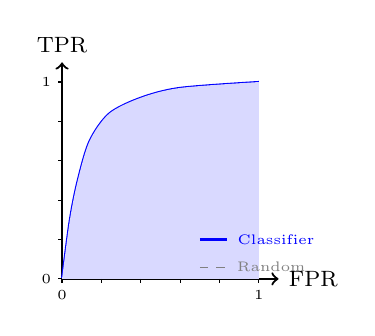
\begin{tikzpicture}[scale=0.5]
    % Axes
    \draw[thick, ->] (0,0) -- (5.5,0) node[right] {\footnotesize FPR};
    \draw[thick, ->] (0,0) -- (0,5.5) node[above] {\footnotesize TPR};

    % Diagonal (random classifier)
    \draw[dashed, gray] (0,0) -- (5,5);

    % ROC curve (good classifier)
    \draw[thick, blue] plot[smooth] coordinates {
        (0,0) (0.2,1.5) (0.4,2.5) (0.7,3.5) (1.2,4.2) (2,4.6) (3,4.85) (5,5)
    };

    % Shaded AUC area
    \fill[blue!15] plot[smooth] coordinates {
        (0,0) (0.2,1.5) (0.4,2.5) (0.7,3.5) (1.2,4.2) (2,4.6) (3,4.85) (5,5)
    } -- (5,0) -- cycle;

    % Axis ticks
    \foreach \x in {0,1,...,5} {
        \draw (\x,0) -- (\x,-0.1);
    }
    \foreach \y in {0,1,...,5} {
        \draw (0,\y) -- (-0.1,\y);
    }

    % Labels
    \node at (0,-0.4) {\tiny 0};
    \node at (5,-0.4) {\tiny 1};
    \node at (-0.4,0) {\tiny 0};
    \node at (-0.4,5) {\tiny 1};

    % Legend
    \draw[thick, blue] (3.5,1) -- (4.2,1) node[right] {\tiny Classifier};
    \draw[dashed, gray] (3.5,0.3) -- (4.2,0.3) node[right] {\tiny Random};
\end{tikzpicture}

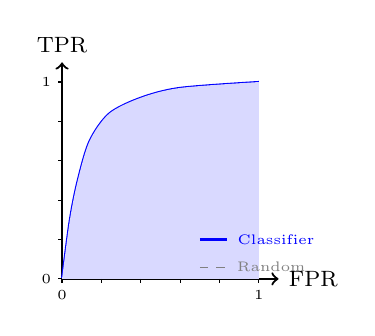
\begin{tikzpicture}[scale=0.5]
    % Axes
    \draw[thick, ->] (0,0) -- (5.5,0) node[right] {\footnotesize FPR};
    \draw[thick, ->] (0,0) -- (0,5.5) node[above] {\footnotesize TPR};

    % Diagonal (random classifier)
    \draw[dashed, gray] (0,0) -- (5,5);

    % ROC curve (good classifier)
    \draw[thick, blue] plot[smooth] coordinates {
        (0,0) (0.2,1.5) (0.4,2.5) (0.7,3.5) (1.2,4.2) (2,4.6) (3,4.85) (5,5)
    };

    % Shaded AUC area
    \fill[blue!15] plot[smooth] coordinates {
        (0,0) (0.2,1.5) (0.4,2.5) (0.7,3.5) (1.2,4.2) (2,4.6) (3,4.85) (5,5)
    } -- (5,0) -- cycle;

    % Axis ticks
    \foreach \x in {0,1,...,5} {
        \draw (\x,0) -- (\x,-0.1);
    }
    \foreach \y in {0,1,...,5} {
        \draw (0,\y) -- (-0.1,\y);
    }

    % Labels
    \node at (0,-0.4) {\tiny 0};
    \node at (5,-0.4) {\tiny 1};
    \node at (-0.4,0) {\tiny 0};
    \node at (-0.4,5) {\tiny 1};

    % Legend
    \draw[thick, blue] (3.5,1) -- (4.2,1) node[right] {\tiny Classifier};
    \draw[dashed, gray] (3.5,0.3) -- (4.2,0.3) node[right] {\tiny Random};
\end{tikzpicture}

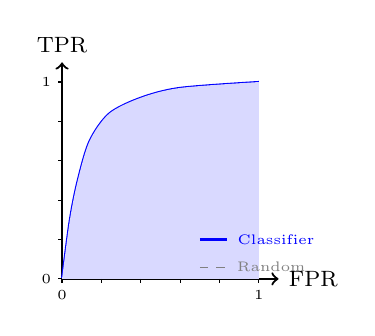
\begin{tikzpicture}[scale=0.5]
    % Axes
    \draw[thick, ->] (0,0) -- (5.5,0) node[right] {\footnotesize FPR};
    \draw[thick, ->] (0,0) -- (0,5.5) node[above] {\footnotesize TPR};

    % Diagonal (random classifier)
    \draw[dashed, gray] (0,0) -- (5,5);

    % ROC curve (good classifier)
    \draw[thick, blue] plot[smooth] coordinates {
        (0,0) (0.2,1.5) (0.4,2.5) (0.7,3.5) (1.2,4.2) (2,4.6) (3,4.85) (5,5)
    };

    % Shaded AUC area
    \fill[blue!15] plot[smooth] coordinates {
        (0,0) (0.2,1.5) (0.4,2.5) (0.7,3.5) (1.2,4.2) (2,4.6) (3,4.85) (5,5)
    } -- (5,0) -- cycle;

    % Axis ticks
    \foreach \x in {0,1,...,5} {
        \draw (\x,0) -- (\x,-0.1);
    }
    \foreach \y in {0,1,...,5} {
        \draw (0,\y) -- (-0.1,\y);
    }

    % Labels
    \node at (0,-0.4) {\tiny 0};
    \node at (5,-0.4) {\tiny 1};
    \node at (-0.4,0) {\tiny 0};
    \node at (-0.4,5) {\tiny 1};

    % Legend
    \draw[thick, blue] (3.5,1) -- (4.2,1) node[right] {\tiny Classifier};
    \draw[dashed, gray] (3.5,0.3) -- (4.2,0.3) node[right] {\tiny Random};
\end{tikzpicture}

    \caption{ROC curve: the blue line shows classifier performance, dashed line is random guessing. Area under curve (AUC) is shaded.}
    \label{fig:roc-curve}
\end{marginfigure}

\begin{lstlisting}[language=Rust]
pub fn auc(roc_points: &[(f64, f64)]) -> f64 {
    let mut area = 0.0;
    for i in 1..roc_points.len() {
        let (x0, y0) = roc_points[i - 1];
        let (x1, y1) = roc_points[i];
        // Trapezoidal rule: width * average height
        area += (x1 - x0) * (y0 + y1) / 2.0;
    }
    area
}
\end{lstlisting}

\begin{keyinsight}
AUC has a probabilistic interpretation: it equals the probability that a
randomly chosen positive (default) is ranked higher than a randomly chosen
negative (non-default).
\end{keyinsight}

\section{Trait-Based Architecture}

Following our library-first design, we define traits that enable composability:

\begin{lstlisting}[language=Rust]
/// Trait for models that produce probability predictions.
pub trait BinaryClassifier {
    fn predict(&self, features: &[f64]) -> bool;
    fn predict_proba(&self, features: &[f64]) -> f64;
}

/// Trait for models that produce raw scores.
pub trait Scorer {
    fn score(&self, features: &[f64]) -> f64;
}
\end{lstlisting}

\marginnote{%
\textbf{Future Benefits}\\[0.3em]
Any classifier implementing \texttt{BinaryClassifier} can be evaluated with our
\func{roc\_curve} and \func{auc} functions.
}

This means our ROC-AUC evaluation works with \emph{any} classifier, not just
\texttt{LinearScorer}. Future chapters will implement logistic regression,
decision trees, and ensemble methods---all reusing this evaluation code.

\section{Results and Analysis}

\subsection{Example Usage}

\begin{lstlisting}[language=bash]
$ cargo run -p qf-02-loan --example loan_analysis
Loading loan applications...
Loaded 10000 applications (850 defaults, 8.5%)

Feature extraction complete.
Training simple scorer (hardcoded weights)...

Evaluation Results:
  AUC: 0.724
  Optimal Threshold: 0.35
  At threshold 0.5:
    Precision: 0.42
    Recall: 0.58
    F1 Score: 0.49
\end{lstlisting}

\subsection{Interpreting the Results}

\begin{itemize}
    \item \textbf{AUC = 0.72}: The model has reasonable discriminative power. It correctly ranks defaults above non-defaults 72\% of the time.
    \item \textbf{Precision = 0.42}: Of predicted defaults, 42\% actually default. Many false alarms.
    \item \textbf{Recall = 0.58}: We catch 58\% of actual defaults. 42\% are missed.
\end{itemize}

\begin{warning}
We used hardcoded weights, not learned weights. Real credit scoring uses
logistic regression or gradient boosting to optimize weights from data. That
comes in later chapters.
\end{warning}

\section{Exercises}

\begin{enumerate}
    \item \textbf{Weight Sensitivity}: Change the weights in \texttt{LinearScorer}. How does AUC change? Which features matter most?

    \item \textbf{Threshold Selection}: Plot precision and recall at various thresholds. Find the threshold that maximizes F1 score.

    \item \textbf{Feature Importance}: Train separate single-feature scorers. Rank features by their individual AUC.

    \item \textbf{Cross-Validation}: Split data into 5 folds. Report mean and standard deviation of AUC across folds.

    \item \textbf{Calibration Plot}: Compare predicted probabilities to actual default rates. Is the model well-calibrated?
\end{enumerate}

\section{Key Takeaways}

\begin{itemize}
    \item \textbf{Feature engineering} transforms raw data into predictive signals
    \item \textbf{One-hot encoding} handles categorical variables
    \item \textbf{Min-max normalization} scales features to comparable ranges
    \item \textbf{Sigmoid} converts scores to probabilities
    \item \textbf{ROC-AUC} evaluates ranking quality, robust to class imbalance
    \item \textbf{Trait-based design} enables reusable evaluation code
\end{itemize}

\vspace{1em}
\noindent\textbf{Next chapter}: Market data fundamentals---OHLCV candlesticks, returns, and simple moving averages.
